%! Licence = CC BY-NC-SA 4.0

%! Author = mariuszindel
%! Date = 06. Jul 2021
%! Project = DS1-Summary

\section{Authentication}

\subsection{Key concepts}
\begin{itemize}
    \item \textbf{Confidentiality:} Protects transmitted data against eavesdropper
    \item \textbf{Integrity:} Provides protection against modification
    \item \textbf{Availability:} Data needs to be available when needed
    \item \textbf{Non-repudiation:} No one can deny an action
    \item \textbf{Identification:} Username connects to a person
    \item \textbf{Authentication:} Verifying a claim of identity with:
    \begin{itemize}
        \item Something you know
        \item Something you have
        \item Something you are
    \end{itemize}
    \item \textbf{Authorization:} Determines what resources a user can access
\end{itemize}

\subsubsection{Time-based One-time Password}
\begin{itemize}
    \item Often used as 2nd factor
    \item Based on keyed-hash message authentication code
\end{itemize}

\subsubsection{Basic Auth}
\begin{itemize}
    \item Load balancer
    \item Services (keep state!)
    \item Only with HTTPS
    \item Can be encoded in URL: \textit{user:pw@domain}
    \item Server will reply with header: \textit{WWW-Authenticate}
\end{itemize}

\subsubsection{Digest Auth}
\begin{itemize}
    \item Based on Basic Auth
    \item Also available in traefik
    \item Hash + nonce, against replay attacks
\end{itemize}
\begin{itemize}[label={\textcolor{ForestGreen}{+}}]
    \item PW not in clear text (MD5), can be SHA-256
    \item Nonce for replay protection for client/server
\end{itemize}
\begin{itemize}[label={\textcolor{red}{--}}]
    \item Browser L\&F
    \item Cannot use scrypt or bcrypt to store PWs
\end{itemize}

\subsubsection{Public/private key}
\begin{itemize}
    \item Create CA
    \item Create certificate
    \item Add nginx security in your local network
\end{itemize}
\begin{center}
    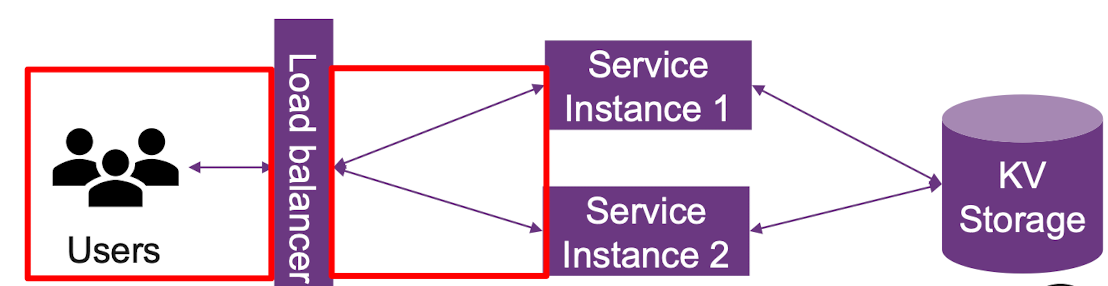
\includegraphics[scale=.3]{05-Auth/Key.png}
\end{center}

\subsubsection{Create SSL CA certificates for server}
\begin{itemize}
    \item Sticky session required
    \item Authenticate in Service Instance
\end{itemize}
\begin{center}
    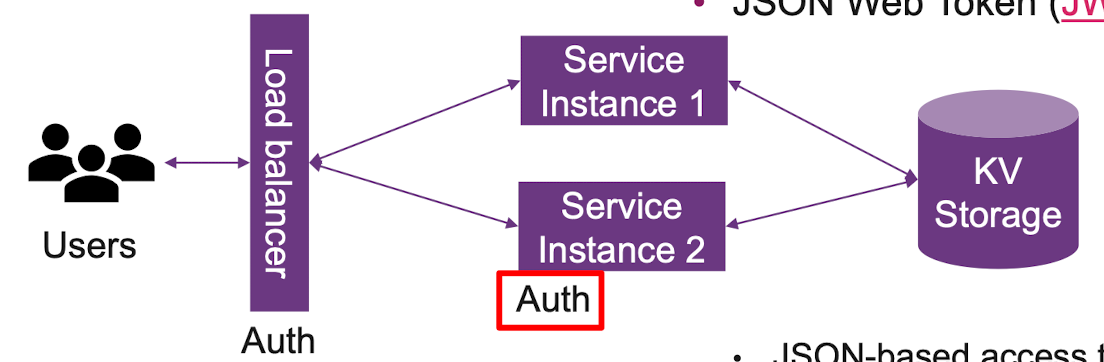
\includegraphics[scale=.3]{05-Auth/sticky-session.png}
\end{center}

\subsubsection{JSON-based access tokens (JWT)}
\begin{itemize}
    \item Stateless
    \item All server instances know a secret token / public key
    \item When user logs in, server send back token
    \item Client sends: Authorization: Bearer <token>
    \item Client can store token in local storage
\end{itemize}
\begin{center}
    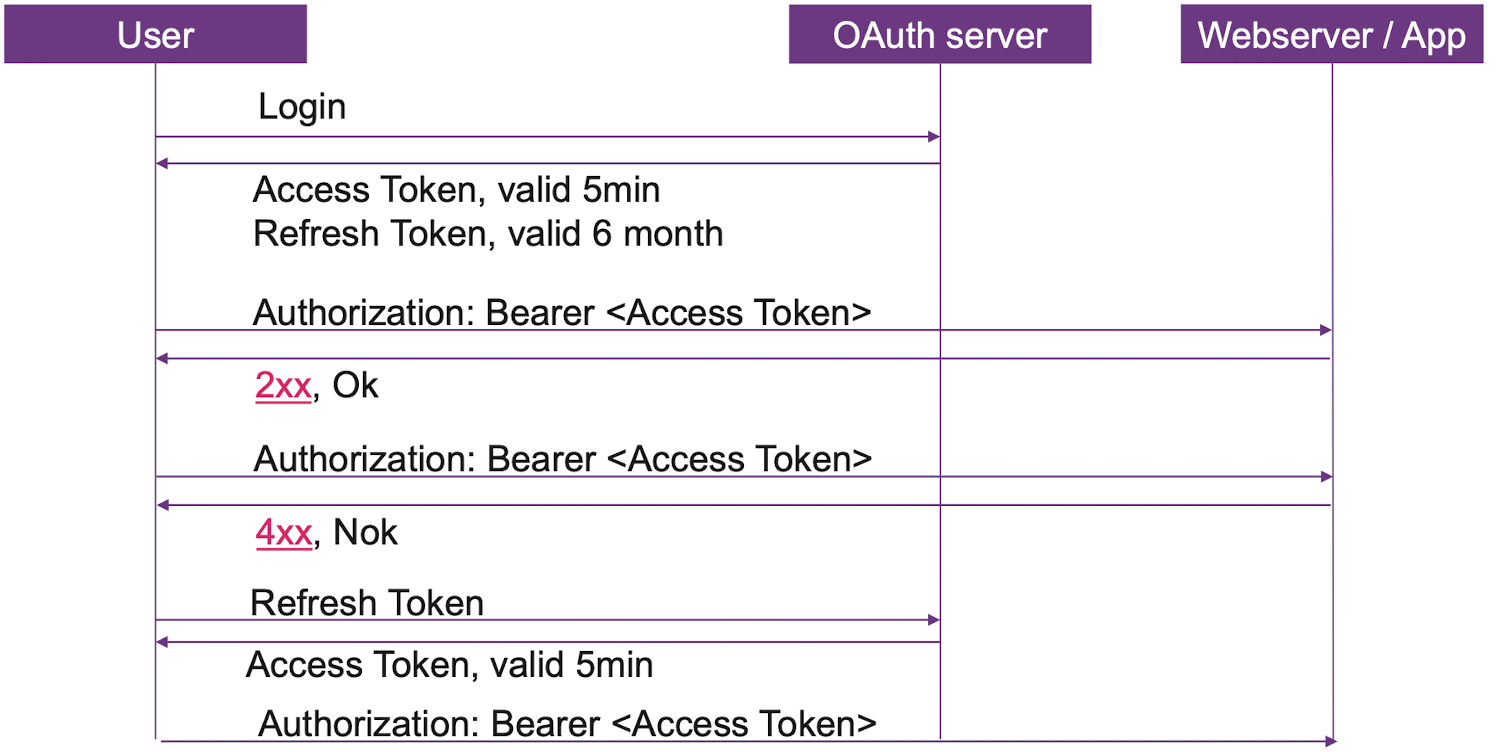
\includegraphics[width=\linewidth]{05-Auth/token.png}    
\end{center}

\paragraph{Access Token}
\begin{itemize}
    \item Short lifetime (10min)
\end{itemize}

\paragraph{Refresh Token}
\begin{itemize}
    \item Used to get a new access token
    \item IAM / Auth server creates access tokens
\end{itemize}
